\chapter{Instrumental Variable Regression}

Our goal with this chapter is to provide an introduction to instrumental variables for mathematicians and statisticians unfamiliar with the topic.
We assume throughout that all random variables are define on the same probability space $ ( \Omega, \mathcal{F}, \prob ) $.
By ``random variable'' we mean scalar or vector valued measurable functions with $ \Omega $ as their domain.\improvement{Rewrite chapter introduction.}
% we turn our attention back to the main application being considered in this thesis: instrumental variable  regression.
% We start by characterizing the type of problem this econometric approach was developed to solve, and then present one of the most well-known and employed\unsure{Is it?} estimation procedures for conducting it: two stages least squares (2SLS).
% Nextly, we show how an IV regression problem can be formulated as a linear inverse problem and discuss the seminal nonparametric method of Newey and Powell \cite{newey2003}, followed by a more recent nonparametric approach called Kernel Instrumental Variable (KIV) \cite{singh2019}.
% We finish with an in-depth analysis of our own method\improvement{Name of the method.}, pointing out its relationship to the others, as well as its strengths and weaknesses.

\section{Endogeneity}

We start by introducing the problem of endogenous covariates.
The structural equation we consider is the following:
\begin{equation}
    \label{eq: structural equation}
    Y = \hstar ( X ) + \varepsilon
,\end{equation}
where $ X $ is a vector of explanatory variables, $ Y $ is the scalar response, $ \varepsilon $ is a zero mean noise and the function $ \hstar $ is the structural parameter we would like to estimate.
The simplest estimation method for this model specification --- and, therefore, one we would like to be able to use --- is ordinary least squares (OLS), which works by finding, within a given class of functions $ \mathcal{H} $, the element which minimizes the mean squared error:
\begin{equation}
    \label{eq: ols estimate}
    \hat{ h } = \argmin_{ h \in \mathcal{H} } \mean [ 
        ( Y - h ( X ) )^2
    ]
.\end{equation}
A reasonable and ample choice for $ \mathcal{H} $ is the set of all square-integrable functions of $ X $, that is, such that $ \mean [ h ( X )^2 ] < \infty $.
Under this choice, we recover the conditional expectation of $ Y $ given $ X $, i.e., $ \hat{ h } ( X ) = \mean [ Y \mid X ] $.
Expanding $ Y $ through (\ref{eq: structural equation}), we find that $ \hat{ h } ( X ) = \hstar ( X ) + \mean [ \varepsilon \mid X ] $.
Hence, if $ \mean [ \varepsilon \mid X ] $ is not identically null, we have introduced bias in our estimation.

This is one of the problems which appear when $ \mean [ \varepsilon \mid X ] \neq 0 $, or, more generally, when $ X $ and $ \varepsilon $ are correlated in some way.
When this happens, we say that $ X $ is \emph{endogenous}.
There are several causes for endogenous covariates, the most common of  which are \cite{wooldridge2001}:
\begin{description}
    \item[Omitted Variables] This means $ \varepsilon $ can be decomposed as $ \gstar ( W ) + \eta $, where $ \mean [ \eta \mid X, W ] = 0 $ a.s. and $ X $ and $ W $ are correlated.
        Hence, when we don't observe $ W $ and leave it to the error term, we end up estimating $ \hstar ( X ) + \mean [ \gstar ( W ) \mid X ] $.
        For example, if we want to regress a persons wage solely on her number of schooling years, there are other variables unaccounted for which influence both wages and schooling, such as natural ability.
        Innately skilled people may tend to be successful in school --- and, therefore, pursue higher levels of education --- as well as show higher performance in their future jobs, resulting in better wages.
    \item[Measurement Error] If we are unable to exactly measure one of the covariates, $ X_{ k } $, and instead measure $ X_{ k }' $ subject to some stochastic error, by using $ X_{ k }' $ in our regression instead of $ X_{ k } $ we are delegating to $ \varepsilon $ some measure of the difference between $ X_{ k } $ and $ X_{ k }' $.
        Depending on how these two variables are related, we may introduce endogeneity.
        For example, $ X_{ k } $ may be a marginal tax rate, but we may only have access to an average tax rate $ X_{ k }' $.
    \item[Simultaneity] Simultaneity arises when one covariate $ X_{ k } $ is determined simultaneously with $ Y $.
        For example, if we are regressing neighborhood murder rates using the size of the local task force as a covariate, there is a simultaneity problem, since larger murder rates in a place cause a larger task force to be allocated there.
\end{description}

Bias in the estimation procedure is only one of the problems which arise when there are endogenous covariates.
It's well known that the OLS estimate for linear regression fails to be consistent if any one of the covariates is endogenous \cite{wooldridge2001}.
To overcome endogeneity a few approaches exist, but by far the one most used by empirical economic research is instrumental variable estimation \cite{wooldridge2001}.

\section{Instrumental Variables}

\begin{deff}
    \label{def: iv}
    An \emph{instrumental variable} for regression problem (\ref{eq: structural equation}) is a random variable $ Z $ such that
    \begin{enumerate}
        \item There is some influence of $ Z $ upon $ X $, that is, the marginal distribution of $ X $ is not the same as the distribution of $ X $ conditioned on $ Z $; \label{en: Z influences X}
        \item The conditional mean of $ \varepsilon $ given $ Z $ is almost surely null, i.e., $ \mean [ \varepsilon \mid Z ] = 0 $. \label{en: Z is exogenous}
    \end{enumerate}
\end{deff}

% \improvement{Causal graph, discuss strength of $ \mean[\varepsilon \mid Z] = 0$, discuss $ Z $ only influences $ Y $ through $ X $.}

The idea behind an instrumental variable is that it is exogenous \ref{en: Z is exogenous} while still influencing $ Y $ through $ X $ \ref{en: Z influences X}.
An exogenous covariate, in contrast to an endogenous one, as a variable that is determined outside of the system described by (\ref{eq: structural equation}).
% The examples ahead will clarify how instrumental variables may be chosen in practice.

Condition \ref{en: Z is exogenous} is only one of the possible meanings for the statement that $ Z $ is exogenous.
Two possible alternatives are requiring that $ Z $ be (1) independent from, or (2) uncorrelated with $ \varepsilon $.
Of course, (1) is a much more strict requirement which implies \ref{en: Z is exogenous}, while (2) is a softer condition, implied by \ref{en: Z is exogenous}.
Independence is almost always impossible to verify in real scenarios, so (1) is not a good option.
In contrast, there are situations where condition (2) is enough for ensuring good properties of IV estimators, including one we will present shortly, the linear model \cite{wooldridge2001}.
However, in order to prepare grounds for the nonparametric methods that will come later, we chose to use the definition which serves both.

Instrumental variables are also studied in the context of causal inference, where the conditions above are presented differently, in terms of causal diagrams.
In this field, instrumental variables are also required that to satisfy a third condition, phrased in terms of the causal diagram describing the relations between variables of interest \cite{hernan2020}:
\begin{enumerate}
    \setcounter{enumi}{2}
    \item All paths from $ Z $ to $ Y $ must pass through $ X $, that is, $ Z $ \emph{only} influences $ Y $ through $ X $.
\end{enumerate}
In this sense, a typical causal diagram for an IV problem is the one in Figure \ref{fig: causal diagram iv}.
\begin{figure}[t]
    \begin{center}
        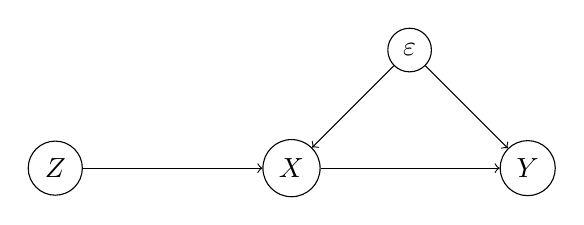
\begin{tikzpicture}[node distance=3cm]
            \node[circle,draw] at (0,0) (X) {$X$};
            \node[circle,draw,right of=X] (Y) {$Y$};
            \node[circle,draw,left of=X] (Z) {$Z$};
            \node[circle,draw,above of=X,xshift=1.5cm,yshift=-1.5cm] (eps) {$\varepsilon$};
            \draw[->] (X) -- (Y);
            \draw[->] (Z) -- (X);
            \draw[->] (eps) -- (X);
            \draw[->] (eps) -- (Y);
        \end{tikzpicture}
    \end{center}
    \caption{Causal diagram for equation (\ref{eq: structural equation}), where $ X $ is endogenous and $ Z $ is an IV.
    Source: prepared by the author.}
    \label{fig: causal diagram iv}
\end{figure}

\section{Two Stages Least Squares (2SLS)}

In this section, we restrict the structural function $ \hstar $ in (\ref{eq: structural equation}) to be affine:
\begin{equation}
    \label{}
    \hstar ( x ) = \beta_{ 0 } + \beta_{ 1 } x_{ 1 } + \cdots + \beta_{ d_{ X } } x_{ d_{ X } }
,\end{equation}
and assume to have access to a random variable $ Z $, taking values in $ \R^{ d_{ Z } } $, satisfying conditions \ref{def: iv} \ref{en: Z influences X} and \ref{en: Z is exogenous}, so that $ Z $ is a valid instrumental variable.
Hence, our data is composed of $ n $ independent joint samples $ \left\{ ( X_{ i }, Z_{ i }, Y_{ i } ) \right\}_{ i=1 }^{ n } $.
Let $ \bX \in \R^{ n \times (d_{ X } + 1) } $ and $ \bZ \in \R^{ n \times ( d_{ Z } + 1 ) } $ be the experiment design matrices with $ 1 $'s in the first column.
